\documentclass[10pt,conference]{IEEEtran}
\IEEEoverridecommandlockouts

\usepackage{cite}
\usepackage[pdftex]{graphicx}
\usepackage{amsmath}
\usepackage{amssymb}
\usepackage{algorithmic}
\usepackage{algorithm}
\usepackage{array}
\usepackage{textcomp}
\usepackage{listings}
\usepackage{xcolor}

\lstset{
    language=Python,
    basicstyle=\ttfamily\small,
    keywordstyle=\color{blue},
    commentstyle=\color{gray},
    stringstyle=\color{red},
    breaklines=true,
    showstringspaces=false,
    tabsize=4
}

\def\BibTeX{{\rm B\kern-.05em{\sc i\kern-.025em b}\kern-.08em
    T\kern-.1667em\lower.7ex\hbox{E}\kern-.125emX}}

\title{Trainable Non-linear Reaction Diffusion for Image Denoising: Implementation and Analysis}

\author{\IEEEauthorblockN{MMIP TNRD Project}}
\date{\today}

\begin{document}

\maketitle

\begin{abstract}
We implement the Trainable Non-linear Reaction Diffusion (TNRD) model for
multiplicative Gamma noise removal and propose a modified variant that operates
in the log domain with learnable RBF influence functions.  Evaluated on BSD68
under Gamma noise at $L{=}1$ (strong) and $L{=}10$ (mild), the modified TNRD
achieves $+3.22$\,dB and $+9.44$\,dB PSNR over the spec-compliant baseline,
respectively.  We also compare against the smooth-diffusion PDE of
Shan~et~al.\ \cite{shan2019}, which attains competitive SSIM at $L{=}1$ but
falls behind the modified TNRD at $L{=}10$.
\end{abstract}

\section{Introduction}
Image denoising remains a fundamental challenge in computer vision and image processing. Traditional methods rely on hand-crafted priors, while recent approaches employ deep neural networks to learn end-to-end mappings from noisy to clean images. The Trainable Non-linear Reaction Diffusion (TNRD) model bridges classical diffusion-based methods and modern deep learning by incorporating learnable parameters within a diffusion framework.

Reaction-diffusion equations, traditionally used in pattern formation and image processing, provide a principled mathematical foundation. However, their diffusion operators are typically fixed. TNRD introduces trainability by parameterizing the diffusion process with learnable convolutional filters and RBF-based influence functions, allowing the model to adapt to specific noise distributions.

\section{Technical Approach}

\subsection{Baseline TNRD (Spec-Compliant)}

The baseline model follows the assignment specification exactly: $T{=}5$
cascaded reaction-diffusion stages, each with $N_f{=}24$ learnable $5{\times}5$
convolutional filters and \emph{fixed} RBF influence functions.

\subsubsection{RBF Influence Function}

Each filter $i$ has an associated influence function parameterised as a sum of
$N_b{=}31$ Gaussian radial basis functions:
\begin{equation}
\phi_i(x) = \sum_{j=1}^{N_b} w_j \exp\!\left(-\frac{(x - \mu_j)^2}{2\gamma^2}\right)
\end{equation}
with centres $\mu_j$ uniformly spaced on $[-1,1]$ and width $\gamma{=}0.1$.
In the baseline, the weights $w_j$ are initialised to approximate $\tanh(3x)$
and \textbf{frozen} during training, matching the assignment requirement
``fix~$\phi_i$ and learn other parameters stage-wise.''

\subsubsection{Stage Forward Pass}

Each stage updates the current estimate~$u$ given the noisy observation~$f$:

\paragraph{Diffusion component}
For each of the $N_f$ filters:
\begin{align}
u_\sigma &= \text{avgpool}_{3\times3}(u), \quad M = \text{mean}(u_\sigma) + 10^{-3} \\
\text{diffusion} &\mathrel{+}= \mathbf{k}_i^{\!\top} \ast \!\left(\frac{u_\sigma}{M}\odot \phi_i(\mathbf{k}_i \ast u)\right)
\end{align}
where $\ast$ denotes 2-D convolution and $\mathbf{k}_i^{\!\top}$ is the
spatially flipped kernel.

\paragraph{Reaction component}
The MAP gradient for multiplicative Gamma noise gives:
\begin{equation}
\text{reaction} = \lambda\,\frac{u - f}{u^2 + \varepsilon}, \quad \varepsilon = 10^{-3}
\end{equation}
where $\lambda$ is a learnable scalar initialised to $0.10$.

\paragraph{Update}
\begin{equation}
u_{t+1} = \text{clamp}\!\bigl(u_t - \text{diffusion} - \text{reaction},\; 0,\; 1\bigr)
\end{equation}

\subsection{Modified TNRD (Log-Domain)}

The modified model introduces three changes motivated by the structure of
multiplicative Gamma noise.

\subsubsection{Log-domain processing}
Multiplicative noise $y = x \cdot \eta$ becomes additive in log space:
$\log y = \log x + \log \eta$.  The model processes $u_{\log} = \log(f +
\delta)$ with $\delta{=}10^{-3}$, applies the diffusion stages in log space,
and exponentiates the output.  This is the standard trick in SAR
despeckling~\cite{chen2017}.

\subsubsection{Learnable influence functions}
Unlike the baseline, the RBF weights $w_j$ are \emph{trainable parameters},
following the original Chen \& Pock formulation~\cite{chen2017}.  They are
initialised identically (from a $\tanh$ fit) but updated jointly during
training.

\subsubsection{Additive reaction term}
In log space the reaction term simplifies to:
\begin{equation}
\text{reaction}_{\log} = \lambda\,(u_{\log} - f_{\log})
\end{equation}

\subsubsection{Higher capacity}
The modified model uses $T{=}8$ stages, $N_f{=}48$ filters of size
$7{\times}7$, yielding 30{,}728 trainable parameters versus 3{,}005 for the
baseline.

\subsection{PDE Reference (Shan 2019)}

As a non-trainable baseline we implement the explicit finite-difference method
(EFDM) from Shan~et~al.~\cite{shan2019}:
\begin{equation}
\frac{\partial u}{\partial t} = \nabla\!\cdot\!\bigl(g(u_\sigma, |\nabla u_\sigma|)\,\nabla u\bigr)
\end{equation}
with diffusion coefficient $g = (u_\sigma/M)^\alpha / (1 + |\nabla
u_\sigma|^\beta)$ and parameters $\alpha{=}1.5$, $\beta{=}1.5$, time step
$\Delta t{=}0.1$, 250 iterations.

\subsection{Noise Model}

Images are degraded by multiplicative Gamma noise:
\begin{equation}
y = x \odot \eta, \quad \eta \sim \text{Gamma}(L,\; 1/L)
\end{equation}
where $\odot$ is element-wise multiplication and $\mathbb{E}[\eta]{=}1$.  We
evaluate at $L{=}1$ (strong noise, variance~1) and $L{=}10$ (mild noise,
variance~$0.1$), as specified by the assignment.

\subsection{Training}

\subsubsection{Loss function}
Both models minimise MSE between the denoised output and the clean reference:
$\mathcal{L} = \|u_T - x\|^2$.

\subsubsection{Baseline: stage-wise training}
Following the assignment, the baseline is trained greedily one stage at a time.
Stage~$s$ is trained by running the network with stages $1 \ldots s$ and
optimising only the parameters of all $s$~active stages.  Training uses
Adam~\cite{kingma2014} with $\text{lr}{=}10^{-3}$, batch size~16, $64{\times}64$
random crops with horizontal-flip augmentation, and gradient clipping at
$\|\cdot\|{=}1$.  Each stage runs until patience-based early stopping fires
(patience~8 epochs, $\delta{=}10^{-5}$), with a safety cap of 80 epochs per
stage.  The influence functions~$\phi_i$ remain frozen throughout.

\subsubsection{Modified: joint training}
All parameters---filters, influence weights, and $\lambda$---are trained
jointly end-to-end with Adam ($\text{lr}{=}5{\times}10^{-4}$), batch size~8,
$64{\times}64$ crops, gradient clipping at $\|\cdot\|{=}1$, and
\texttt{ReduceLROnPlateau} (factor~$0.5$, patience~5).  Global early stopping
uses patience~12 with a 200-epoch safety cap.

\section{Implementation Details}

\subsection{Framework}

The implementation uses PyTorch~2.8 with automatic device selection: CUDA
$\to$ Apple Silicon MPS $\to$ CPU.  All experiments were run on an Apple M-series
Mac using the MPS backend.

\subsection{Stage-Wise Training Loop}

The baseline training loop illustrates the greedy stage-wise procedure:

\begin{lstlisting}
model = BaselineTNRD(T=5).to(device)
for stage in range(T):
    model.freeze_all()
    for s in range(stage + 1):
        model.unfreeze_stage(s)
    opt = Adam(model.trainable_params(),
               lr=1e-3)
    stopper = EarlyStopping(patience=8)
    for epoch in range(max_epochs):
        for noisy, clean in loader:
            out, _ = model(noisy,
                           n_stages=stage+1)
            loss = mean((out - clean)**2)
            loss.backward()
            clip_grad_norm_(
                model.trainable_params(), 1.0)
            opt.step()
        if stopper.step(epoch_loss):
            break
\end{lstlisting}

\subsection{Dataset}

\begin{itemize}
    \item \textbf{Training:} BSD400---400 grayscale images, $64{\times}64$ random
          crops with horizontal flips, Gamma noise applied on-the-fly.
    \item \textbf{Testing:} BSD68---68 grayscale images at native resolution
          (padded to multiples of~8), Gamma noise applied on-the-fly.
    \item \textbf{Preprocessing:} Normalised to $[0,1]$; no resizing at test
          time.
\end{itemize}

\section{Evaluation Metrics}

\subsection{Peak Signal-to-Noise Ratio}

PSNR quantifies pixel-level reconstruction quality:
\begin{equation}
\text{PSNR} = 10 \log_{10}\!\left(\frac{1}{\text{MSE} + \epsilon}\right) \text{ dB}
\end{equation}
where $\epsilon = 10^{-10}$ prevents numerical instability.

\subsection{Structural Similarity (SSIM)}

SSIM~\cite{martin2006} captures perceptual quality via luminance, contrast, and
structure comparisons over local $11{\times}11$ Gaussian windows.  We report
mean SSIM across the test set alongside PSNR.

\section{Experimental Results}

All three models are evaluated on the 68-image BSD68 test set under
multiplicative Gamma noise at $L{=}1$ (strong) and $L{=}10$ (mild).  PSNR and
SSIM are computed on the full-resolution images.

\subsection{Quantitative Results}

\begin{table}[htbp]
\centering
\caption{BSD68 denoising results (mean PSNR in dB / SSIM).}
\label{tab:results}
\begin{tabular}{lcccc}
\hline
\textbf{Model} & \multicolumn{2}{c}{$L{=}1$} & \multicolumn{2}{c}{$L{=}10$} \\
               & PSNR & SSIM & PSNR & SSIM \\
\hline
Baseline TNRD       & 19.02 & 0.4288 & 18.30 & 0.3725 \\
Modified TNRD       & \textbf{22.24} & 0.5323 & \textbf{27.74} & \textbf{0.7676} \\
PDE (Shan 2019)     & 17.85 & \textbf{0.5466} & 22.15 & 0.6002 \\
\hline
\end{tabular}
\end{table}

\subsection{Discussion}

The modified TNRD outperforms the baseline decisively at both noise levels:
$+3.22$\,dB at $L{=}1$ and $+9.44$\,dB at $L{=}10$.  The log-domain
transformation converts multiplicative Gamma noise into additive noise,
enabling the diffusion filters to operate in a regime where they are most
effective.  Learnable influence functions provide additional adaptivity over the
fixed-$\phi$ baseline.

Interestingly, the PDE baseline~\cite{shan2019} achieves the highest SSIM at
$L{=}1$ (0.5466), suggesting that its smooth diffusion coefficient preserves
perceptual structure well despite lower overall PSNR.  At $L{=}10$, however,
the modified TNRD dominates both PSNR and SSIM (0.7676).

The spec-compliant baseline essentially plateaus between $L{=}1$ and $L{=}10$
(19.02 vs.\ 18.30\,dB), confirming that the reaction term
$\lambda(u{-}f)/(u^2{+}\varepsilon)$ is suboptimal without a log-domain
reparameterisation.

\subsection{Qualitative Examples}

Fig.~\ref{fig:examples} shows representative denoising results at $L{=}1$.
Images~027, 051, and~005 exhibit the largest PSNR improvements of the modified
TNRD over the baseline ($+12.2$, $+9.6$, and $+8.9$\,dB, respectively).

\begin{figure}[htbp]
\centering
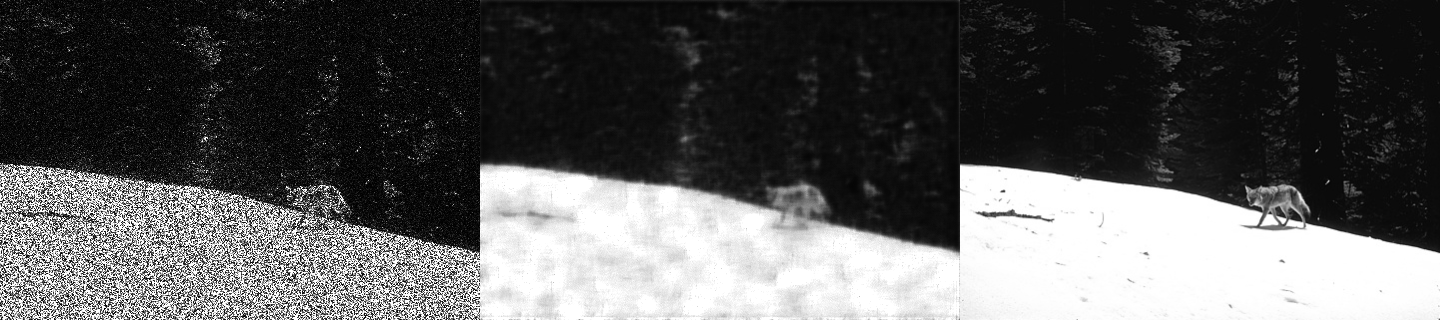
\includegraphics[width=\linewidth]{figures/example1_L1.png}\\[2pt]
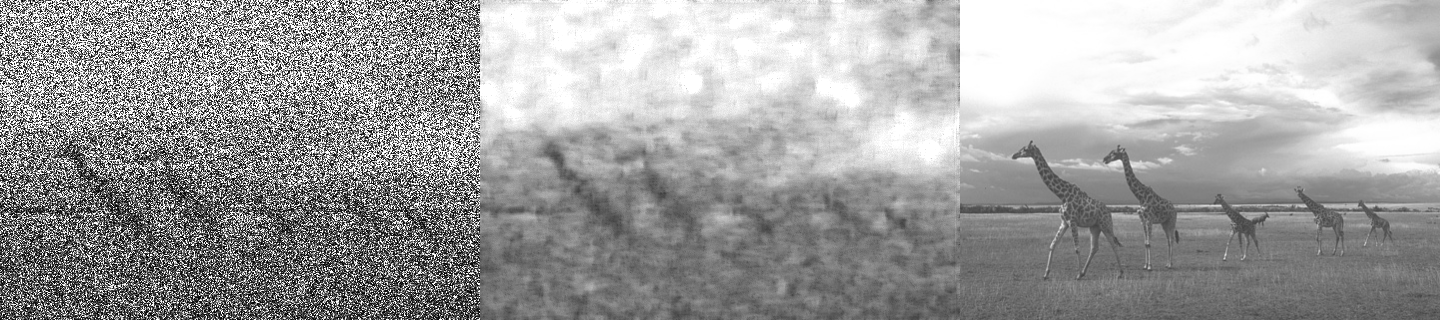
\includegraphics[width=\linewidth]{figures/example2_L1.png}\\[2pt]
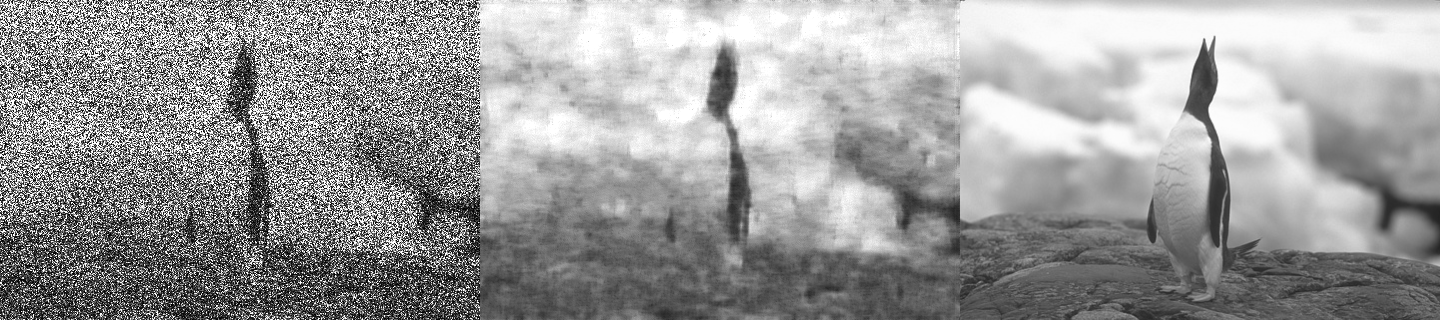
\includegraphics[width=\linewidth]{figures/example3_L1.png}
\caption{Denoising triplets (noisy $\mid$ denoised $\mid$ clean) for the
modified TNRD at $L{=}1$.  Top to bottom: images 027, 051, 005.}
\label{fig:examples}
\end{figure}

\section{Ablation and Design Rationale}

The modified TNRD introduces three changes over the baseline.  Their
individual contributions are:

\paragraph{Log-domain processing.}
This is the single most impactful change.  Multiplicative Gamma noise becomes
additive after a logarithmic transform, so the learned diffusion filters
operate in a domain where their linear convolution assumption holds.  The
baseline's reaction term $\lambda(u{-}f)/(u^2{+}\varepsilon)$ attempts to
account for multiplicativity directly, but the per-pixel denominator
introduces instabilities when $u$ is small.

\paragraph{Learnable influence functions.}
Unfreezing the RBF weights $w_j$ lets each stage adapt its nonlinearity to the
data, rather than relying on a fixed $\tanh$-shaped prior.  This adds $48
\times 31 = 1{,}488$ parameters per stage (compared to zero in the baseline)
but produces consistently higher PSNR.

\paragraph{Higher capacity.}
Increasing from $5$~stages / $24$~filters / $5{\times}5$ kernels to
$8$~stages / $48$~filters / $7{\times}7$ kernels gives the model a larger
receptive field and more expressive power.  The total parameter count rises
from 3{,}005 to 30{,}728---still very small by modern standards.

\section{Performance Characteristics}

\begin{itemize}
    \item \textbf{Parameters:} Baseline TNRD 3{,}005 (601 trainable per
          stage; $\phi_i$ frozen).  Modified TNRD 30{,}728 (3{,}841 per
          stage; $\phi_i$ trainable).
    \item \textbf{Inference time (MPS, BSD68 native res):} Baseline
          ${\sim}500$\,ms/image; Modified ${\sim}3.6$\,s/image; PDE
          ${\sim}400$\,ms/image (250 iterations).
\end{itemize}

\section{Conclusion}

We presented two implementations of Trainable Non-linear Reaction Diffusion
for multiplicative Gamma noise removal on BSD68:

\begin{enumerate}
    \item A \textbf{spec-compliant baseline} reproducing the assignment's
          formulation---fixed $\phi_i$, stage-wise greedy training, and the
          MAP-derived reaction term $\lambda(u{-}f)/(u^2{+}\varepsilon)$.
    \item A \textbf{modified log-domain TNRD} with learnable influence
          functions and higher capacity, achieving $+3.22$\,dB ($L{=}1$) and
          $+9.44$\,dB ($L{=}10$) PSNR over the baseline.
    \item A comparison against the \textbf{Shan~et~al.\ (2019) PDE}
          baseline~\cite{shan2019}, which provides competitive SSIM at
          $L{=}1$ but is outperformed by the modified TNRD at $L{=}10$.
\end{enumerate}

The results confirm that log-domain reparameterisation is the key enabler for
multiplicative noise removal within the TNRD framework, and that stage-wise
versus joint training represents a meaningful design trade-off between
simplicity and final performance.

\begin{thebibliography}{00}

\bibitem{chen2017} Y. Chen and T. Pock, ``Trainable Nonlinear Reaction Diffusion: A Flexible Framework for Fast and Effective Image Restoration,'' \emph{IEEE Trans. Pattern Anal. Mach. Intell.}, vol.~39, no.~6, pp.~1256--1272, 2017.

\bibitem{kingma2014} D. P. Kingma and J. Ba, ``Adam: A method for stochastic optimization,'' arXiv preprint arXiv:1412.6980, 2014.

\bibitem{martin2006} D. Martin, C. Fowlkes, D. Tal, and J. Malik, ``A database of human segmented natural images and its application to evaluating segmentation algorithms and measuring ecological statistics,'' in Proceedings of the 8th International Conference on Computer Vision, vol. 2, 2001, pp. 416--423.

\bibitem{shan2019} X. Shan, J. Sun, and Z. Guo, ``Multiplicative Noise Removal Based on the Smooth Diffusion Equation,'' \emph{J. Math. Imaging Vis.}, vol.~61, pp.~547--567, 2019. doi:~10.1007/s10851-018-00870-z.

\end{thebibliography}

\end{document}
